\documentclass{article}
\usepackage{amsmath}
\usepackage[mathletters]{ucs}
\usepackage[utf8x]{inputenc}
\usepackage[margin=1.5in]{geometry}
\usepackage{enumerate}
\newtheorem{theorem}{Theorem}
\usepackage[dvipsnames]{xcolor}
\usepackage{pgfplots}
\setlength{\parindent}{0cm}
\usepackage{graphics}
\usepackage{graphicx} % Required for including images
\usepackage{subcaption}
\usepackage{bigintcalc}
\usepackage{pythonhighlight} %for pythonkode \begin{python}   \end{python}
\usepackage{appendix}
\usepackage{arydshln}
\usepackage{physics}
\usepackage{tikz-cd}
\usepackage{booktabs} 
\usepackage{adjustbox}
\usepackage{mdframed}
\usepackage{relsize}
\usepackage{physics}
\usepackage[thinc]{esdiff}
\usepackage{fixltx2e}
\usepackage{esint}  %for lukket-linje-integral
\usepackage{xfrac} %for sfrac
\usepackage{hyperref} %for linker, må ha med hypersetup
\usepackage[noabbrev, nameinlink]{cleveref} % to be loaded after hyperref
\usepackage{amssymb} %\mathbb{R} for reelle tall, \mathcal{B} for "matte"-font
\usepackage{listings} %for kode/lstlisting
\usepackage{verbatim}
\usepackage{graphicx,wrapfig,lipsum,caption} %for wrapping av bilder
\usepackage{mathtools} %for \abs{x}
\usepackage[norsk]{babel}
\definecolor{codegreen}{rgb}{0,0.6,0}
\definecolor{codegray}{rgb}{0.5,0.5,0.5}
\definecolor{codepurple}{rgb}{0.58,0,0.82}
\definecolor{backcolour}{rgb}{0.95,0.95,0.92}
\lstdefinestyle{mystyle}{
    backgroundcolor=\color{backcolour},   
    commentstyle=\color{codegreen},
    keywordstyle=\color{magenta},
    numberstyle=\tiny\color{codegray},
    stringstyle=\color{codepurple},
    basicstyle=\ttfamily\footnotesize,
    breakatwhitespace=false,         
    breaklines=true,                 
    captionpos=b,                    
    keepspaces=true,                 
    numbers=left,                    
    numbersep=5pt,                  
    showspaces=false,                
    showstringspaces=false,
    showtabs=false,                  
    tabsize=2
}

\lstset{style=mystyle}
\author{Oskar Idland}
\title{Oblig 8}
\date{}
\begin{document}
\maketitle
\newpage
\section*{\underline{A Diskusjonsoppgaver}}
\subsection*{Oppgave 1}
\subsubsection*{a)}
Hvis $E < qV_0$ vil ikke ringen kunne krysset gapet og vil vil reise tilbake der den kom fra

\subsubsection*{b)}
Hvis $E > qV_0$ vil ringen krysset gapet og fortsette å bevege seg på den andre siden. 

\subsubsection*{c)}
Hvis vi gjentar dette 100 ganger med $E < qV_0 $ vil ringen reise tilbake der den kom fra 100/100 ganger. 

\subsubsection*{d)}
Hvis $E < V_0$ vil majoriteten av elektronene ikke krysse over til område C, men bli sendt tilbake der de kom fra. 
Hvis $E > V_0$ vil alle elektronene krysse over til område C.

\subsubsection*{e)}


\begin{figure}[h!]
    \centering
    \begin{subfigure}{.4\textwidth}
      \centering
      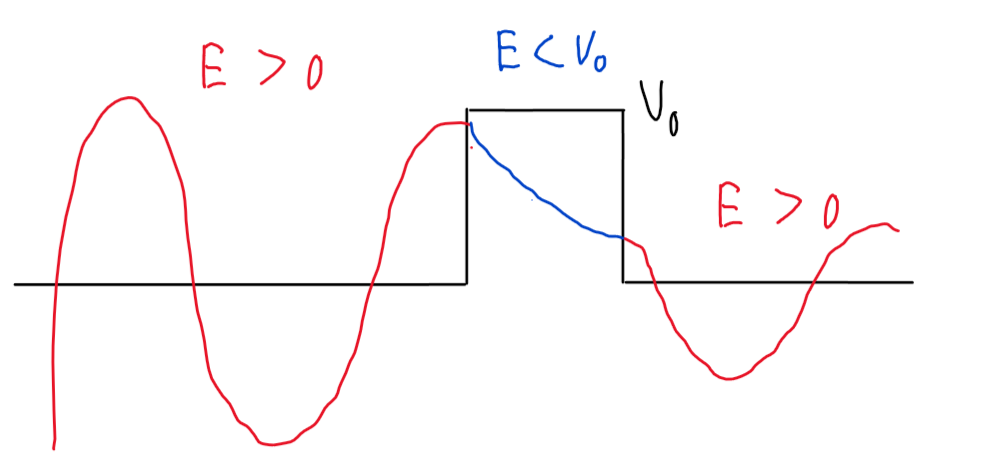
\includegraphics[width = \textwidth]{1.e.1.png}
      \caption{Skisse av bølgefunksjonen med energi $E$ som reiser over potensialet $V_0$, hvor $E<V_0$}
      \label{subfig: 1.e.1}
    \end{subfigure}
    \hfill
    \begin{subfigure}{.4\textwidth}
      \centering
      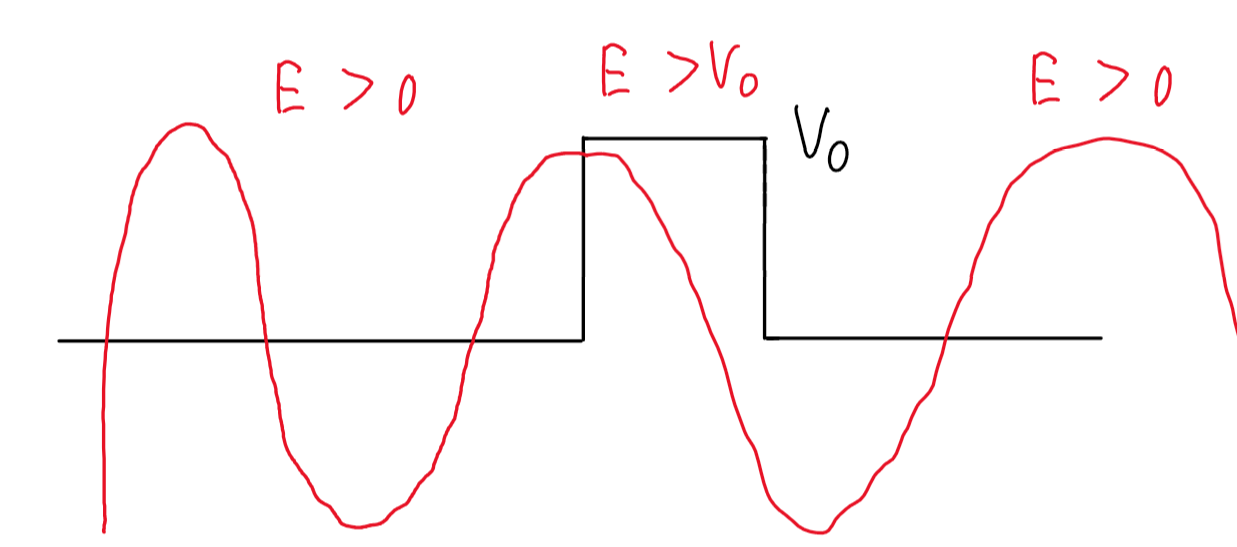
\includegraphics[width = \textwidth]{1.e.2.png}
      \caption{Skisse av bølgefunksjonen med energi $E$ som reiser over potensialet $V_0$ hvor $E>V_0$}
      \label{subfig: 1.e.2}
    \end{subfigure}
    \hfill
    \caption{To scenario hvor energien $E$ til elektronene er både større og mindre enn potensialet $V_0$. I begge tilfeller er bølgelengden konstant både før og etter å ha reist over $V_0$.}
    \label{fig: 1.e}
\end{figure}


\subsection*{Oppgave 2}
Riktig svar er påstand A. \underline{$ψ$ har samme bølgelengde på begge sider av barrieren}. 
Ettersom bølgefunksjonen er på formen $ψ(x) = Ae^{ikx} + Be^{-ikx}$, med forskjellige koeffisienter $A$ og $B$ før, inni og etter barrieren vil den ha samme bølgelengde på begge sider av barrieren, men varierende amplitude. 


\section*{\underline{B Regenoppgaver}}



\end{document}